% !TeX program = xelatex
% Отчёт по лабораторной работе №20. Сборка: make
\documentclass[variant=labwork]{bsuir}

\usepackage{graphicx}
\usepackage{float}
\usepackage{needspace}
\usepackage{fvextra}
\usepackage{tikz}
\usetikzlibrary{calc}

\newcommand{\imgplaceholder}[1]{%
  \fbox{\parbox{0.88\textwidth}{\centering\vspace{1.3cm}\textit{[Рисунок: #1]}\vspace{1.3cm}}}%
}

\DefineVerbatimEnvironment{code}{Verbatim}{
    breaklines=true,
    breakanywhere=true,
    fontsize=\fontsize{10pt}{12pt}\selectfont
}
\sloppy
\setlength{\emergencystretch}{2em}

\let\origthebibliography\thebibliography
\renewcommand{\thebibliography}[1]{%
  \origthebibliography{#1}%
  \small%
  \setlength{\itemsep}{1pt}%
  \setlength{\parsep}{0pt}%
}

\setlist[itemize]{
    label=--,
    leftmargin=0pt,
    itemindent=1.4\parindent,
    labelindent=1.4\parindent,
    labelsep=0.5em,
    topsep=0pt,
    itemsep=0pt,
    parsep=0pt
}
\setlist[enumerate]{
    label=\arabic*,
    leftmargin=0pt,
    itemindent=1.5\parindent,
    labelindent=1.5\parindent,
    labelsep=0.5em,
    topsep=0pt,
    itemsep=0pt,
    parsep=0pt
}

\titlecontents{section}[12pt]{}
    {\thecontentslabel\hspace{0.5em}}
    {}{\titlerule*[4pt]{.}\thecontentspage}

\faculty{Компьютерного проектирования}
\departmentlong{Инженерной психологии и эргономики}
\departmentshort{ИПиЭ}
\coursename{Интерфейсы информационных систем}
\manager{Прудник А.М.}
\workcode{20}
\worktitle{Разработка структуры веб-приложения на Angular с использованием модулей, компонентов и сервисов}
\titlepageyear{2026}
\group{310102}
\student{Кадол А.П.}
\titleright{}
\titleleft{}

\renewcommand{\thefigure}{\arabic{figure}}
\renewcommand{\thetable}{\arabic{table}}
\renewcommand{\theequation}{\arabic{equation}}

\begin{document}
\maketitle
\mainmatter

\textbf{Цель работы:} получить практические навыки создания базовой архитектуры веб-приложения на Angular: модуль, компоненты и сервис с внедрением зависимостей.

\textbf{Исходные данные.}
Тематический вариант совпадает с лабораторной работой №\,1: блоговая платформа Folio. В макете уже заданы тёмно-зелёная шапка, бумажный фон, карточка статьи шириной до 360~px и графические ассеты (логотип, аватар, иконки, обложки). По заданию этой работы в Angular переносятся три компонента и один сервис. Поля объекта статьи: \texttt{id}, \texttt{title}, \texttt{author}, \texttt{previewText}, \texttt{imageUrl}. Состав приложения приведён в таблице~\ref{tab:arch}.

\begin{longtable}{|>{\raggedright\arraybackslash}p{\dimexpr(\textwidth-6\tabcolsep-4\arrayrulewidth)*4/10\relax}|>{\centering\arraybackslash}p{\dimexpr(\textwidth-6\tabcolsep-4\arrayrulewidth)*3/10\relax}|>{\raggedright\arraybackslash}p{\dimexpr(\textwidth-6\tabcolsep-4\arrayrulewidth)*3/10\relax}|}
  \caption{Состав Angular-приложения}
  \label{tab:arch}\\
  \hline
  Сущность & Декоратор & Назначение \\
  \hline
  \endfirsthead
  \multicolumn{3}{l}{Продолжение таблицы~\thetable}\\
  \hline
  Сущность & Декоратор & Назначение \\
  \hline
  \endhead
  \texttt{AppModule} & \texttt{@NgModule} & Объявляет компоненты и запускает приложение \\
  \hline
  \texttt{HeaderComponent} & \texttt{@Component} & Шапка с логотипом Folio \\
  \hline
  \texttt{ArticleListComponent} & \texttt{@Component} & Лента: данные сервиса и цикл \texttt{*ngFor} \\
  \hline
  \texttt{ArticleCardComponent} & \texttt{@Component} & Одна карточка, вход \texttt{@Input() article} \\
  \hline
  \texttt{ArticlesService} & \texttt{@Injectable} & Метод \texttt{getData()} с mock-статьями \\
  \hline
\end{longtable}

\textbf{Теоретические сведения.}
Модуль \texttt{@NgModule} собирает декларации компонентов, импорты и точку входа. Компонент \texttt{@Component} связывает класс, шаблон и файл стилей; стили по умолчанию инкапсулированы и не протекают в соседние компоненты. Сервис с \texttt{providedIn: 'root'} создаётся один на всё приложение. Список получает его через параметр конструктора, а в \texttt{ngOnInit} забирает массив. Карточка не ходит в сервис сама: родитель передаёт один элемент привязкой свойства, а карточка объявляет это свойство через \texttt{@Input()}.

\textbf{Ход выполнения работы.}
Проект собран в каталоге \texttt{my-app} на ветке \texttt{angular}, ветка \texttt{main} с прототипом на Vue не изменялась. Команда \texttt{ng new my-app} выполнена с отключённым standalone-режимом, чтобы появился \texttt{AppModule}, а не набор самостоятельных компонентов. Компоненты и сервис созданы через Angular CLI: \texttt{ng generate component} для \texttt{header}, \texttt{article-card} и \texttt{article-list}, \texttt{ng generate service} для \texttt{articles}.

\texttt{ArticlesService} помечен \texttt{@Injectable(\{ providedIn: 'root' \})} и не указан в \texttt{providers} модуля: корень приложения и есть область видимости синглтона. Метод \texttt{getData()} возвращает три объекта. Тексты первых двух статей взяты из данных прототипа, третья продолжает ту же ленту. Обложки лежат в \texttt{src/assets} и подключены в \texttt{angular.json}, потому что сборщик Angular~19 сам по себе не копирует этот каталог. Состав mock-данных приведён в таблице~\ref{tab:articles}.

\begin{longtable}{|>{\centering\arraybackslash}p{\dimexpr(\textwidth-6\tabcolsep-4\arrayrulewidth)*1/10\relax}|>{\raggedright\arraybackslash}p{\dimexpr(\textwidth-6\tabcolsep-4\arrayrulewidth)*6/10\relax}|>{\raggedright\arraybackslash}p{\dimexpr(\textwidth-6\tabcolsep-4\arrayrulewidth)*3/10\relax}|}
  \caption{Статьи, которые возвращает \texttt{getData()}}
  \label{tab:articles}\\
  \hline
  id & Заголовок & Автор \\
  \hline
  \endfirsthead
  \multicolumn{3}{l}{Продолжение таблицы~\thetable}\\
  \hline
  id & Заголовок & Автор \\
  \hline
  \endhead
  1 & Утренние страницы: ритуал, который возвращает голос & Анна Волкова \\
  \hline
  2 & Как писать, когда не хочется писать & Пётр Лебедев \\
  \hline
  3 & Редактура как чтение вслух & Мария Соколова \\
  \hline
\end{longtable}

\texttt{ArticleListComponent} принимает сервис в конструкторе (\texttt{private articlesService: ArticlesService}) и в \texttt{ngOnInit} сохраняет результат \texttt{getData()} в поле \texttt{articles}. Шаблон списка перебирает массив директивой \texttt{*ngFor} и для каждого элемента создаёт \texttt{app-article-card} с привязкой \texttt{[article]="article"}. В карточке то же имя объявлено как \texttt{@Input() article}. Шаблон карточки выводит обложку, заголовок, лид и автора; аватар и ряд Like / Comment / Share взяты из ассетов макета и не являются полями сервиса.

Стили разложены по файлам \texttt{*.component.css}: шапка, сетка ленты и карточка не делят один файл. Общие токены цвета и шрифтов (Inter и Playfair Display, фон \texttt{\#FAF6F1}, бренд \texttt{\#0F3D3A}) заданы в \texttt{styles.css}, чтобы компоненты пользовались теми же переменными, что и макет. Общий вид ленты показан на рисунке~\ref{fig:feed}, третья карточка целиком~--- на рисунке~\ref{fig:card}, узкая ширина~--- на рисунке~\ref{fig:mobile}.

\begin{figure}[H]
  \centering
  
\includegraphics[width=0.92\textwidth]{screenshots/feed.png}
  \caption{Лента Folio: шапка и карточки из сервиса}
  \label{fig:feed}
\end{figure}

\begin{figure}[H]
  \centering
  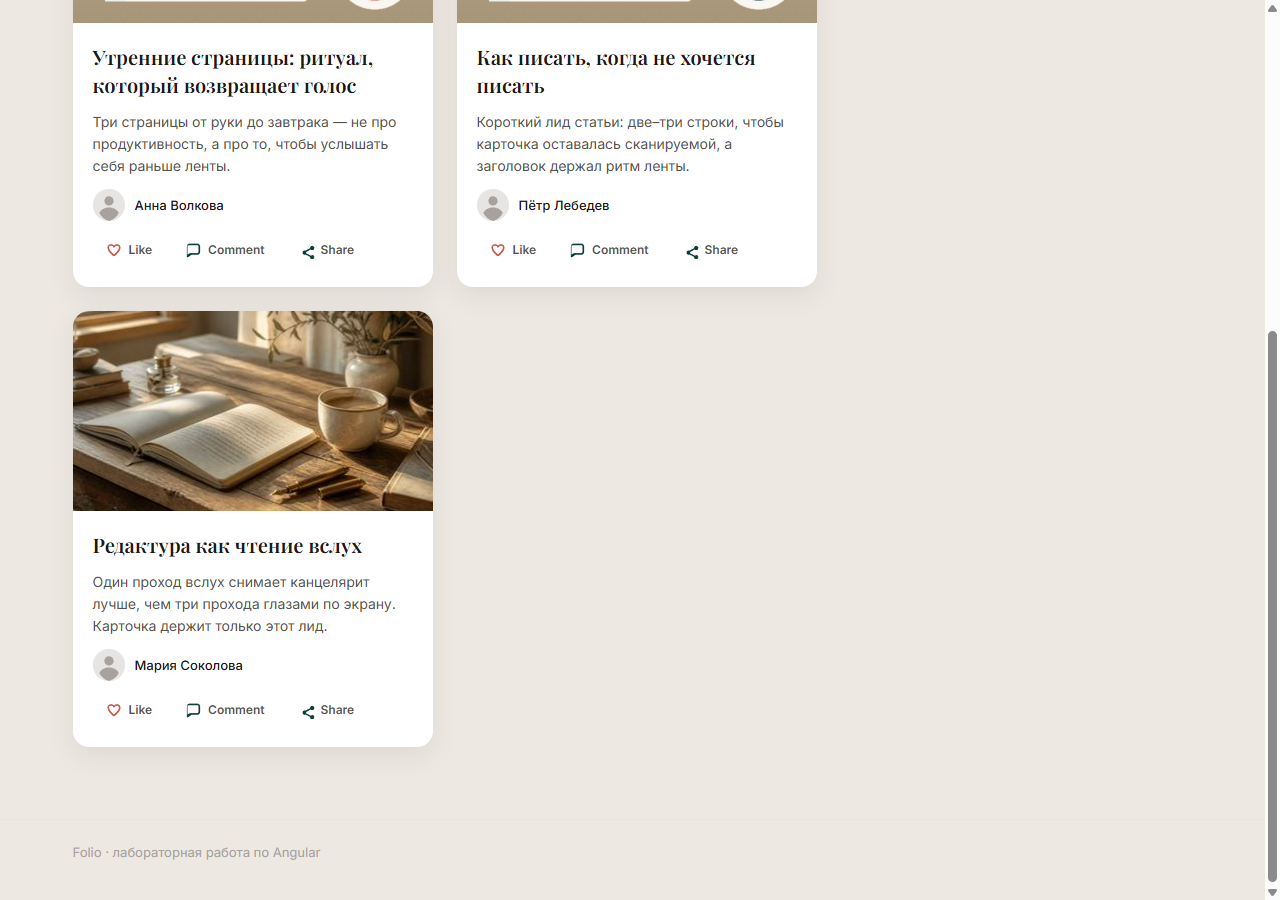
\includegraphics[width=0.92\textwidth]{screenshots/card.png}
  \caption{Третья статья списка и подвал страницы}
  \label{fig:card}
\end{figure}

\begin{figure}[H]
  \centering
  
\includegraphics[width=0.42\textwidth]{screenshots/feed-mobile.png}
  \caption{Та же лента при ширине 390~px}
  \label{fig:mobile}
\end{figure}

Запуск описан в \texttt{README.md}: из каталога \texttt{my-app} выполняются \texttt{npm install} и \texttt{npm start}, после чего приложение доступно по адресу \texttt{http://localhost:4200/}.

\textbf{Вывод:} базовый каркас блога Folio собран на Angular. Модуль объявляет три компонента, сервис в корне приложения отдаёт mock-статьи, список получает их через конструктор и \texttt{ngOnInit}, а карточка рисует один элемент по \texttt{@Input}. Внешний вид повторяет макет лабораторной работы №\,1: те же токены, логотип и обложки.

\end{document}
